\chapter{Clasificación de imágenes}

Esta clase tiene como objetivo comprender los conceptos de clasificación espectral utilizando algoritmos de clustering. Para ello se clasificá una imagen de la zona de la Triple Frontera.

\section{Clasificación por k-means}

Abra la imagen

\begin{center}
\directory{LC08\_224-078\_2018-01-05.dim}.
\end{center}

diríjase luego a
\begin{center}
\menu{Raster > Classification > Unsupervised classification > K-Means cluster analysis}
\end{center}

En la pestaña \menu{I/O Parameters} seleccione la imagen, el nombre de salida y la carpeta donde guardará el resultado (Figura \ref{fig:kmeans}). Presione \menu{Run} para finalizar.

\begin{figure}[h!]
    \centering
    \subfloat[1-I/O Parameters]{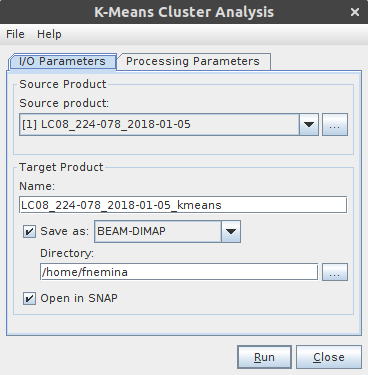
\includegraphics[width=0.4\textwidth]{fig:kmeans1.png}\label{fig:kmeans1}}
    \hspace{1cm}
    \subfloat[Processing parameters]{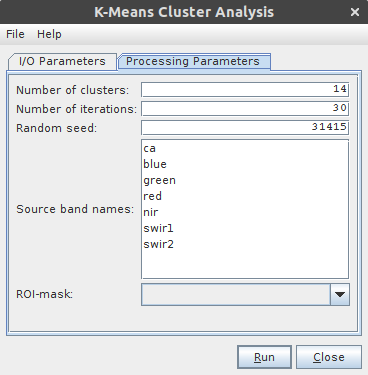
\includegraphics[width=0.4\textwidth]{fig:kmeans2.png}\label{fig:kmeans2}}
    \caption{Clasificación de imágenes por el método \emph{k-means}.}
    \label{fig:kmeans}
\end{figure}

Obtendrá una imagen clasificada en el \menu{Product explorer}. Despliegue la banda \emph{class\_indices}.

Podrá verlos nombres de las clases y su centroide en \emph{Index Codings, Cluster\_classes}, dentro de la imagen.

\section{Reclasificación}


El producto obtenido representa las clases espectrales encontradas por el metodo de clasificación. Para generar la imagen con las clases informacionales, es necesario reclasificarla asignando un nombre y color a cada clase espectral.

Comience desplegando en simultaneo la imagen clasificada y la original, en una combinación de bandas conveniente. Seleccione la imagen clasificada y haga click en \menu{View > Tool windows > Colour manipulation}. Aparecerála lista de clases espectrales (Figura \ref{fig:colman}).

\begin{figure}[h!]
    \centering
    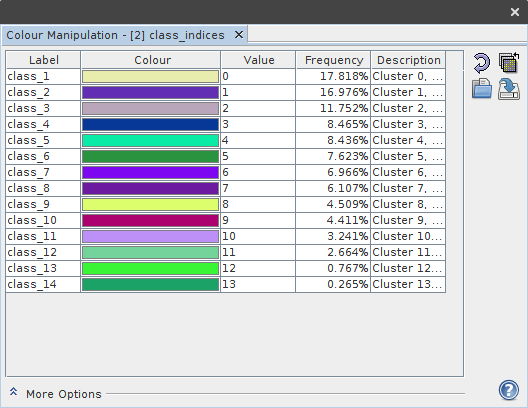
\includegraphics[width=0.4\textwidth]{fig:colman.png}
    \caption{Herramienta para asignar colores en la imagen.}
    \label{fig:colman}
\end{figure}

Una forma sencilla de reconocer cada clase espectral en la imagen, es asignarle un color contrastante. Cambie el color haciendo click sobre la celda del color. En el menú desplegable elija, por ejemplo rojo o amarillo y verifique que el resto de las clases no lo tenga. Identifique a que uso o cobertura pertenece, comparándola con la imagen sin clasificar. Modifique el nombre de la columna \emph{Label} por los que figuran en la columna \emph{Codigo} (Tabla \ref{tab:usos}). Vuelva a cambiar el color de la clase identificada a negro y repita el procedimiento para el resto.

Una vez terminado el procedimiento, asigne a cada categoría de uso y cobertura el color que figura en la tabla . Guarde la imagen con los cambios, haga click derecho sobre el nombre y presione en \menu{Save product} (Figura \ref{fig:resclass}).

\begin{table}[hbt]
    \centering
    \begin{tabular}{p{11cm}cc}
        \toprule
        Nombre & Codigo & Color (R,G,B) \\
        \midrule
        Áreas terrestres cultivadas y manejada & A11 & \textcolor{A11}{$\blacksquare$}\texttt{178,223,138}
        \\
        Vegetación natural y semi-natural & A12 & \textcolor{A12}{$\blacksquare$}\texttt{51,160,44}\\
        Áreas acuáticas o regularmente inundadas cultivadas & A23  &
        \textcolor{A23}{$\blacksquare$}\texttt{253,191,111}\\
        Vegetación natural y semi-natural acuática o
	regularmente inundadas & A24 & \textcolor{A24}{$\blacksquare$}\texttt{255,127,0}\\
        Superficies artificiales y áreas asociadas & B15  &
        \textcolor{B15}{$\blacksquare$}\texttt{251,154,153}\\
        Áreas descubiertas o desnudas & B16 & \textcolor{B16}{$\blacksquare$}\texttt{227,26,28}\\
        Cuerpos artificiales de agua, nieve y hielo & B27 &
        \textcolor{B27}{$\blacksquare$}\texttt{166,206,227}\\
        Cuerpos naturales de agua, nieve y hielo & B28&
        \textcolor{B28}{$\blacksquare$}\texttt{31,120,180}\\
        \bottomrule
    \end{tabular}
\caption{\label{tab:usos}Categorias usos del suelo segun el esquema LCCS2 de la FAO.}
\end{table}

\begin{figure}[h!]
    \centering
    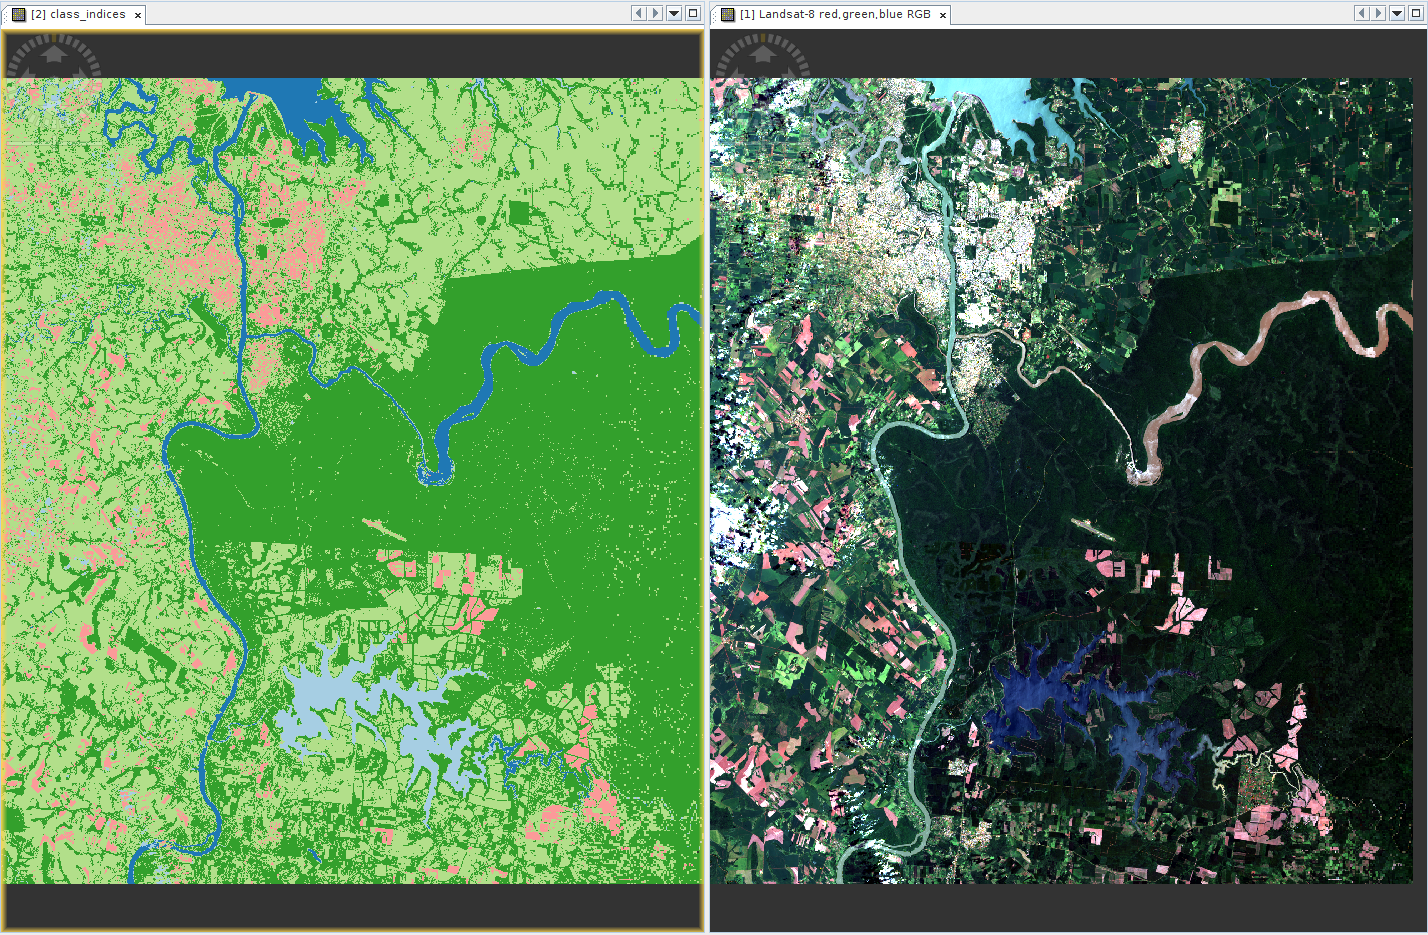
\includegraphics[width=0.7\textwidth]{fig:reclass.png}
    \caption{Imagen reclasificada junto a la imagen en color real.}
    \label{fig:resclass}
\end{figure}


Puede observar el porcentaje de cada clase espectral en la columna \emph{Frequency} en la pestaña \menu{Colour manipulation}.

\section{Parámetros de clasificación}

Para mejorar la clasificación, es posible cambiar cuatro parámetros en la pestaña \menu{Processing parameters} del \menu{ K-Means cluster analysis} (Figura \ref{fig:kmeans2}).

\begin{itemize}
  \item \emph{Number of clusters}: El número de clases espectrales en la que se clasificará la imagen.
  \item \emph{Number of iterations}: El número de veces que se repetirá el proceso de k-means, si no hubiera convergencia antes.
  \item \emph{Random seed}: La semilla que se utiliza para asignar las clases iniciales de forma aleatoria.
  \item \emph{Source band names}: Bandas para la clasificación. En caso de no seleccionar alguna/s en particular, se utilizaran todas.
\end{itemize}

\section{Exportar visualización}

En el SNAP es posible exportar la vista como imagen y utilizarla en otro software. Para ello, diríjase a \menu{File > Export > Other > View as image}. Seleccione si quiere exportar la región que está viendo (\emph{View region}) o toda la imagen (\emph{Full scene}) y el formato de archivo (Figura \ref{fig:vista}).

\begin{figure}[h!]
    \centering
    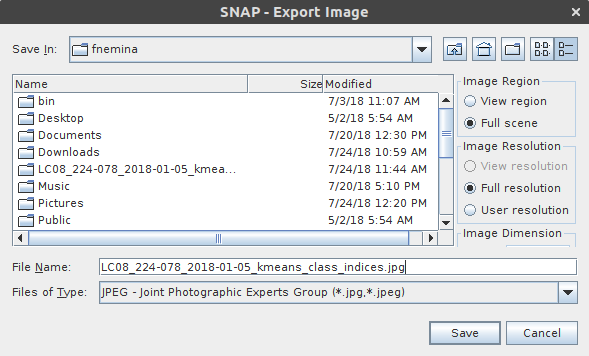
\includegraphics[width=0.5\textwidth]{fig:vista.png}
    \caption{Herramienta para exportar la vista de la imagen.}
    \label{fig:vista}
\end{figure}

Para mantener la georreferenciación elija el formato de archivo \emph{GeoTIFF - TIFF with geo-location}.

Para exportar la vista como KMZ, primero deberá reproyectar la imagen a coordenadas geográficas. En este caso, tendrá que reasignar los colores a cada clase espectral. La herramienta a utilizar es \menu{File > Export > Other > View as Google Earth KMZ}.


\section{Actividad práctica}

\begin{enumerate}
  \item Clasifique la imagen con los siguientes Parámetros
  \begin{table}[h]
  \centering
  \begin{tabular}{cccl}
  \toprule
  Number of clusters & Number of iterations & Random seed & Source band name \\ \midrule
  7                  & 30                   & 31415       & Todas            \\
  14                 & 30                   & 31415       & Todas            \\
  14                 & 30                   & 198674      & Todas            \\
  28                 & 30                   & 31415       & Todas            \\
  28                 & 60                   & 31415       & Todas            \\
  14                 & 30                   & 31415       & blue,green,red   \\
  14                 & 30                   & 31415       & red,nir,swir1    \\ \bottomrule
  \end{tabular}
  \end{table}
  \item ¿Qué sucede con la clasificación al aumentar el número de clusters? ¿Y al aumentar el número de iteraciones?
  \item A mismo número de clusters ¿qué bandas conviene utilizar: \emph{blue, green, red} o \emph{red, nir,swir1}? ¿Puede explicarlo en términos de las coberturas de la imagen?
  \item ¿Que parámetros elegiría para una mejor clasificación de la zona?
\end{enumerate}

Estas preguntas y actividades no serán evaluadas. Su objetivo es discutirlas en el foro de consultas e intercambio de la clase.
